\documentclass[8pt,a4paper,compress]{beamer}

\usepackage{/home/siyer/lib/slides}

\title{Analysis of Algorithms}
\date{}

\begin{document}
\begin{frame}
\vfill
\titlepage
\end{frame}

\begin{frame}
\frametitle{Outline}
\tableofcontents
\end{frame}

\section{Complexity of Algorithms}
\begin{frame}[fragile]
\begin{itemize}
\item people writing programs to process large amounts of data are invariably led to the following questions:
\begin{itemize}
\item how long will my program take, ie, what is the time complexity of my program?
\item how much memory will my program need, ie, what is the space complexity of my program?
\end{itemize}
\end{itemize}
\end{frame}

\section{Time Complexity}
\begin{frame}[fragile]
\begin{itemize}
\item running example (3-sum problem)
\begin{lstlisting}[language=Java]
public class ThreeSum {
    public static int count(int[] a) {
        int N = a.length;
        int cnt = 0;
        for (int i = 0; i < N; i++) {
            for (int j = i+1; j < N; j++) {
                for (int k = j+1; k < N; k++) {
                    if (a[i] + a[j] + a[k] == 0) {
                        cnt++;
                    }
                }
            }
        }
        return cnt;
    }
    
    public static void main(String[] args)  { 
        In in = new In(args[0]);
        int[] a = in.readAllInts();
        Stopwatch timer = new Stopwatch();
        int cnt = count(a);
        StdOut.println("elapsed time = " + timer.elapsedTime());
        StdOut.println(cnt);
    } 
}
\end{lstlisting}

\begin{lstlisting}[language={}]
$ java ThreeSum 1Kints.txt 
elapsed time = 0.334
70
$ java ThreeSum 2Kints.txt 
elapsed time = 2.637
528
\end{lstlisting}
\end{itemize}
\end{frame}

\subsection*{Experimental Analysis}
\begin{frame}[fragile]
\begin{itemize}
\item \lstinline{Stopwatch} API
\begin{lstlisting}[language={}]
public class Stopwatch

    Stopwatch()          // create a stopwatch
    double elapsedTime() // return elapsed time since creation
    ...
\end{lstlisting}

\item \lstinline{Stopwatch} client
\begin{lstlisting}[language=Java]
public class ThreeSum {
    ...
    public static void main(String[] args)  { 
        In in = new In(args[0]);
        int[] a = in.readAllInts();
        Stopwatch timer = new Stopwatch();
        int cnt = count(a);
        StdOut.println("elapsed time = " + timer.elapsedTime());
        StdOut.println(cnt);
    } 
}
\end{lstlisting}

\begin{lstlisting}[language={}]
$ java ThreeSum 1Kints.txt 
elapsed time = 0.335
70
\end{lstlisting}

\item \lstinline{Stopwatch} implementation
\begin{lstlisting}[language=Java]
public class Stopwatch {
    private final long start;
    
    public Stopwatch() { start = System.currentTimeMillis(); }
    
    public double elapsedTime() {
        return (System.currentTimeMillis() - start) / 1000.0;
    }
}
\end{lstlisting}
\end{itemize}
\end{frame}

\begin{frame}[fragile]
\begin{itemize}
\item a more sophisticated \lstinline{Stopwatch} client that produces experimental data for \lstinline{ThreeSum}
\begin{lstlisting}[language=Java]
public class DoublingTest {
    public static double timeTrial(int N) {
        int MAX = 1000000;
        int[] a = new int[N];
        for (int i = 0; i < N; i++) {
            a[i] = StdRandom.uniform(-MAX, MAX);
        }
        Stopwatch timer = new Stopwatch();
        ThreeSum.count(a);
        return timer.elapsedTime();
    }

    public static void main(String[] args) { 
        for (int N = 250; true; N += N) {
            double time = timeTrial(N);
            StdOut.printf("%7d %5.1f\n", N, time);
        } 
    } 
} 
\end{lstlisting}

\begin{lstlisting}[language={}]
$ java DoublingTest
    250   0.0
    500   0.0
   1000   0.1
   2000   0.8
   4000   6.4
   8000  51.1
... 
\end{lstlisting}
\end{itemize}
\end{frame}

\begin{frame}[fragile]
\begin{itemize}
\item plots of the experimental data 
\begin{center}
\includegraphics[scale=0.45]{{./figures/threesum}.pdf}
\end{center}

\item from the log-log plot we have $$\lg T(N) = 3\lg N + \lg a,$$ where $a$ is a constant

$$\therefore \text{\ \ \ \ } T(N)=aN^3$$ 
and since $T(8000)=51.1$, we have $$T(N)=9.98\times 10^{-11}N^3$$
\end{itemize}
\end{frame}

\begin{frame}[fragile]
\begin{itemize}
\item doubling-ratio experiments
\begin{lstlisting}[language=Java]
public class DoublingRatio {
    public static double timeTrial(int N) {
        int MAX = 1000000;
        int[] a = new int[N];
        for (int i = 0; i < N; i++) {
            a[i] = StdRandom.uniform(-MAX, MAX);
        }
        Stopwatch timer = new Stopwatch();
        ThreeSum.count(a);
        return timer.elapsedTime();
    }

    public static void main(String[] args) { 
        double prev = timeTrial(125);
        for (int N = 250; true; N += N) {
            double time = timeTrial(N);
            StdOut.printf("%6d %7.1f %5.1f\n", N, time, time / prev);
            prev = time;
        } 
    } 
} 
\end{lstlisting}

\begin{lstlisting}[language={}]
$ java DoublingRatio
   250   0.0   2.7
   500   0.0   4.8
  1000   0.1   6.9
  2000   0.8   7.7
  4000   6.4   8.0
  8000  51.1   8.0
...
\end{lstlisting}
\end{itemize}
\end{frame}

\subsection*{Mathematical Analysis}
\begin{frame}[fragile]
\begin{itemize}
\item the total running time of a program is determined by: the cost of executing each statement (property of the computer); and the frequency of execution of each statement (property of the program and the input)

\item we write $\sim f(N)$ (called tilde approximation) to represent any function that, when divided by $f(N)$, approaches 1 as $N$ grows, and we write $g(N)\sim f(N)$ to indicate that $g(N)/f(N)$ approaches 1 as $N$ grows

\item most often, we work with tilde approximations of the form $g(N)\sim af(N)$ where $f(N)=N^b(\log N)^c$ with $a, b$, and $c$ constants and refer to $f(N)$ as the order of growth of $g(N)$
\end{itemize}
\end{frame}

\begin{frame}[fragile]
\begin{itemize}
\item analyzing the running time of \lstinline{ThreeSum.count()}
\begin{lstlisting}[language=Java, mathescape]
public static int count(int[] a) {
    int N = a.length;                           $[A]$
    int cnt = 0;
    for (int i = 0; i < N; i++) {               $[B]$ 
        for (int j = i+1; j < N; j++) {         $[C]$
            for (int k = j+1; k < N; k++) {     $[D]$
                if (a[i] + a[j] + a[k] == 0) {
                    cnt++;                      $[E]$
                }
            }
        }
    }
    return cnt;
}
\end{lstlisting}
\begin{center}
\begin{tabular}{cccc}
\textbf{statement block} & \textbf{time} & \textbf{frequency} & \textbf{total time}\\ \hline \\
$[E]$ & $t_0$ & $x$ (depends on input) & $t_0x$ \\
$[D]$ & $t_1$ & $N^3/6-N^2/2+N/3$  & $t_1(N^3/6-N^2/2+N/3)$ \\
$[C]$ & $t_2$ & $N^2/2-N/2$  & $t_2(N^2/2-N/2)$ \\
$[B]$ & $t_3$ & $N$  & $t_3N$ \\
$[A]$ & $t_4$ & $1$  & $t_4$ 
\end{tabular} 
\end{center}
grand total: $(t_1/6)N^3+(t_2/2-t_1/2)N^2+(t_1/3-t_2/2+t_3)N+t_4+t_0x$

tilde approximation: $\sim(t_1/6)N^3$ (assuming $x$ is small)

order of growth: $N^3$
\end{itemize}
\end{frame}

\begin{frame}[fragile]
\begin{itemize}
\item for many programs, developing a mathematical model of running time reduces to the following steps
\begin{itemize}
\item develop an input model, including a definition of the problem size
\item identify the inner loop
\item define a cost model that includes operations in the inner loop
\item determine the frequency of execution of those operations for the given input
\end{itemize}

\item for \lstinline{ThreeSum}, the input model is $N$ numbers; the inner loop is the statements in a triply nested \lstinline{for} loop; the cost model is the number of array accesses; and the number of array accesses is $N^3/2$
\end{itemize}
\end{frame}

\begin{frame}[fragile]
\begin{itemize}
\item commonly encountered functions in analysis of algorithms
\begin{center}
\begin{tabular}{ccc}
\textbf{description} & \textbf{notation} & \textbf{definition} \\ \hline \\
floor & $\floor{x}$ & largest integer not greater than $x$ \\
ceiling & $\ceil{x}$ & smallest integer not smaller than $x$ \\
natural logarithm & $\ln N$ & $\log_eN$ ($x$ such that $e^x=N$) \\ 
binary logarithm & $\lg N$ & $\log_2N$ ($x$ such that $2^x=N$) \\
integer binary logarithm & $\floor{\lg N}$ & largest integer not greater than $\lg N$ \\
harmonic numbers & $H_N$ & $1+1/2+1/3+\dots+1/N$ \\
factorial & $N!$ & $1\times 2\times 3\times \dots \times N$
\end{tabular} 
\end{center}

\item useful approximations for analysis of algorithms
\begin{center}
\begin{tabular}{ccc}
\textbf{description} & \textbf{approximation} \\ \hline \\
harmonic sum & $H_N=1+1/2+1/3+\dots+1/N \approx \ln N$ \\
triangular sum & $1+2+3+\dots+N \approx N^2/2$ \\
geometric sum & $1+2+4+8+\dots+N=2N-1 \approx 2N$ when $N=2^n$ \\
Stirling's approximation & $\log N! = \log 1 +\log 2 + \log 3 + \dots + \log N \approx N\log N$ \\
binomial coefficients & $\binom{N}{K}\approx N^k/k!$ where $k$ is a small constant \\
exponential &  $(1-1/x)^x \approx 1/e$
\end{tabular} 
\end{center}
\end{itemize}
\end{frame}

\begin{frame}[fragile]
\begin{itemize}
\item order-of-growth classifications
\begin{center}
\begin{tabular}{cccc}
\textbf{description} & \textbf{function} & \textbf{code description} & \textbf{example} \\ \hline \\
constant & 1 & statement & add two numbers \\
logarithmic & $\log N$ & divide in half & binary search \\
linear & $N$ & loop & find the maximum \\
linearithmic & $N\log N$ & divide and conquer & merge sort \\
quadratic & $N^2$ & double loop & check all pairs \\
cubic & $N^3$ & triple loop & check all triples \\
exponential & $2^N$ & exhaustive search & check all subsets
\end{tabular} 
\end{center}
\begin{center}
\includegraphics[scale=0.4]{{./figures/order_of_growth}.pdf}
\end{center}
\end{itemize}
\end{frame}

\begin{frame}[fragile]
\begin{itemize}
\item predictions on the basis of order-of-growth functions for a program that takes a few hours for input of size $N$
\begin{center}
\begin{tabular}{ccccc}
\textbf{description} & \textbf{function} & \textbf{$2x$ factor} & \textbf{$10N$} & \textbf{$10N$ on $10x$ CPU}\\ \hline \\
linear & $N$ & 2 & a day & a few hours \\
linearithmic & $N\log N$ & 2 & a day & a few hours \\
quadratic & $N^2$ & 4 & a few weeks & a day \\
cubic & $N^3$ & 8 & several months & a few weeks \\
exponential & $2^N$ & $2^N$ & never & never
\end{tabular} 
\end{center}
\end{itemize}
\end{frame}


\subsection*{Designing Faster Algorithms}
\begin{frame}[fragile]
\begin{itemize}
\item search problem: search for a key in a collection of $N$ keys

\item linear search
\begin{lstlisting}[language=Java]
public static int rank(int key, int[] a) {
    for (int i = 0; i < a.length; i++) {
        if (a[i] == key) { return i; }
    }
    return -1;
}
\end{lstlisting}

order of growth: $N$
 
\item binary search
\begin{center}
\includegraphics[scale=0.65]{./figures/bs1.pdf}

\smallskip

successful search for the key 23
\end{center}
\end{itemize}
\end{frame}

\begin{frame}[fragile]
\begin{itemize}
\item binary search
\begin{center}
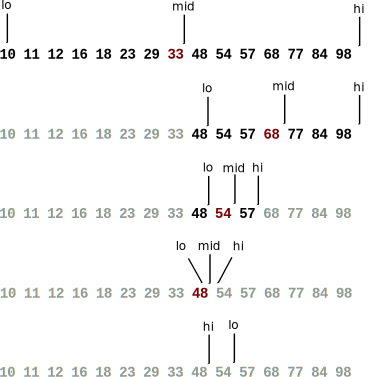
\includegraphics[scale=0.65]{./figures/bs2.pdf}

\smallskip

unsuccessful search for the key 50
\end{center}
\end{itemize}
\end{frame}

\begin{frame}[fragile]
\begin{itemize}
\item binary search and whitelisting
\begin{lstlisting}[language=Java]
public class BinarySearch {
    public static int rank(int key, int[] a) {
        int lo = 0;
        int hi = a.length - 1;
        while (lo <= hi) {
            int mid = lo + (hi - lo) / 2;
            if (key < a[mid]) { hi = mid - 1; }
            else if (key > a[mid]) { lo = mid + 1; }
            else { return mid; }
        }
        return -1;
    }

    public static void main(String[] args) {
        In in = new In(args[0]);
        int[] whitelist = in.readAllInts();
        Arrays.sort(whitelist);
        while (!StdIn.isEmpty()) {
            int key = StdIn.readInt();
            if (rank(key, whitelist) == -1) {
                StdOut.println(key);
            }
        }
    }
}
\end{lstlisting}
\end{itemize}
\end{frame}

\begin{frame}[fragile]
\begin{itemize}
\item binary search and whitelisting
\begin{lstlisting}[language={}]
tinyW.txt tinyT.txt
   84        23
   48        50
   68        10
   10        99
   18        18
   98        23
   12        98
   23        84
   54        11
   57        10
   48        48
   33        77
   16        13
   77        54
   11        98
   29        77
             77
             68
\end{lstlisting}

\begin{lstlisting}[language={}]
$ java BinarySearch tinyW.txt < tinyT.txt
50
99
13
\end{lstlisting}

binary search order of growth: $\lg N + 1$ 

whitelisting order of growth: $M(\lg N + 1)$, where $M$ is the number of calls to \lstinline{rank()}
\end{itemize}
\end{frame}

\begin{frame}[fragile]
\begin{itemize}
\item faster solution to the 3-sum problem
\begin{lstlisting}[language=Java]
import java.util.Arrays;

public class ThreeSumFast {
    public static int count(int[] a) {
        Arrays.sort(a);
        int N = a.length;
        int cnt = 0;
        for (int i = 0; i < N; i++) {
            for (int j = i + 1; j < N; j++) {
                if (BinarySearch.rank(-a[i] - a[j], a) > j) {
                    cnt++;
                }
            }
        }
        return cnt;
    }
    
    public static void main(String[] args) {
        In in = new In(args[0]);
        int[] a = in.readAllInts();
        StdOut.println(count(a));
    }
}
\end{lstlisting}

order of growth: $N^2\log N$
\end{itemize}
\end{frame}

\subsection*{Caveats}
\begin{frame}[fragile]
\begin{itemize}
\item with leading-term approximations, we ignore constant coefficients in lower-order terms, which may not be justifed

\item the assumption that the inner loop dominates may not always be correct 

\item the assumption that each instruction always takes the same amount of time is not always correct

\item typically, there are many things going on in your computer and these can affect the reproducibility of experiments

\item often, when we compare two different programs for the same task, one might be faster in some situations, and slower in others

\item when running time is sensitive to inputs, we may get inconsistent results or be unable to validate our hypotheses

\item we have been focusing on measuring performance as a function of a single parameter, generally the size of the input, but it is not unusual to have several parameters
\end{itemize}
\end{frame}

\subsection*{Coping With Dependence on Inputs}
\begin{frame}[fragile]
\begin{itemize}
\item carefully model the kind of input to be processed in the problems that we need to solve

\item take an extremely pessimistic view of the performance of algorithms, and seek the running time in the worst case

\item an important way to provide a performance guarantee is to introduce randomness

\item for many applications, the algorithm ``input'' might be not just data, but the sequence of operations performed by the client

\item amortize the cost by keeping track of the total cost of all operations, divided by the number of operations
\end{itemize}
\end{frame}

\section{Space Complexity}
\begin{frame}[fragile]
\begin{itemize}
\item memory requirements for primitive types
\begin{center}
\begin{tabular}{cc}
\textbf{type} & \textbf{bytes} \\ \hline \\
\lstinline$boolean$ & 1 \\
\lstinline$byte$ & 1 \\
\lstinline$char$ & 2 \\
\lstinline$int$ & 4 \\
\lstinline$float$ & 4 \\
\lstinline$long$ & 8 \\
\lstinline$double$ & 8
\end{tabular} 
\end{center}

\item to determine the memory usage of an object, we add the amount of memory used by each instance variable to the overhead associated with each object, which is 16 bytes

\item a \lstinline{Counter} object uses 32 bytes: 16 bytes of overhead, 8 bytes for its \lstinline{String} instance variable (a reference), 4 bytes for its \lstinline{int} instance variable, and 4 bytes of padding

\item a nested non-static (inner) class requires an extra 8 bytes of overhead (for reference to the enclosing instance)
\end{itemize}
\end{frame}

\begin{frame}[fragile]
\begin{itemize}
\item an array of primitive-type values typically requires 24 bytes of header information (16 bytes of object overhead, 4 bytes for the length, and 4 bytes of padding) plus the memory needed to store the values

\item an array of $N$ \lstinline{int} values uses $24 + 4N$ bytes 

\item an array of objects is an array of references to objects, so we need to add the space for the references to the space required for the objects

\item an array of $N$ \lstinline{Date} objects uses 24 bytes (array overhead) plus $8N$ bytes (references) plus 32 bytes for each object, for a grand total of $24+40N$ bytes

\item a two-dimensional array is an array of arrays (each array is an object)

\item a two-dimensional $M$-by-$N$ array of \lstinline{double} values uses 24 bytes (overhead for array of arrays) plus $8M$ bytes (references to the row arrays) plus $24M$ bytes (overhead from the row arrays) plus $8MN$ bytes (for the $N$ \lstinline{double} values in each of the $M$ rows) for a grand total of $8MN+32M+24\sim 8MN$ bytes
\end{itemize}
\end{frame}


\begin{frame}[fragile]
\begin{itemize}
\item a \lstinline{String} object uses a total of 40 bytes: 16 bytes for object overhead plus 4 bytes for each of the three \lstinline{int} instance variables (an offset into a character array, string length, and a hash code that saves recomputation) plus 8 bytes for the array reference plus 4 bytes of padding


\item a \lstinline{String} of length $N$ typically uses 40 bytes (for the \lstinline{String} object) plus $24+2N$ bytes (for the array that contains the characters) for a
total of $64+2N$ bytes

\item when you use the \lstinline{substring()} method, you create a new \lstinline{String} object (40 bytes) but reuse the same character (\lstinline{value[]}) array, so a substring of an existing string takes just 40 bytes
\end{itemize}
\end{frame}
\end{document}
